\chapter{Hermes}
\label{cap:hermes}

O Hermes \cite{renan2021hermes} é um interceptador de mensagens, entre o cliente e servidor. O Hermes é encarregado de ordenar as mensagens usando algoritmos de consenso. Após ordenadas as mensagens, o Hermes entrega as mensagens aos servidores replicados.

O objetivo do Hermes é abstrair os detalhes da ordenação de requisições em sistemas replicados em arquiteturas de microsserviços. Trata-se de um conjunto de interfaces que visam oferecer uma camada de abstração. O Hermes usa o padrão de projetos \textit{proxy}, uma vez que as requisições chegam até o Kubernetes, o serviço do Hermes as intercepta e faz o tratamento de obter consenso entre as réplicas. O cliente envia as requisições para o Hermes, mas isso fica transparente ao usuário. O módulo Hermes utiliza a biblioteca \textit{Hashicorp Raft}\footnote{Hashicorp Raft: \url{https://github.com/hashicorp/raft}}.

% \textbf{Hermes}

O Hermes tem propósitos de ser desacoplado, escalável e compartimentado em tecnologia de contêiner Docker e orquestrado em Kubernetes. Utilizar o Kubernetes é parte do mecanismo de interceptação e também serve para fazer gestão das réplicas. O sistema usufrui de mecanismos do Kubernetes que isolam as réplicas em seus \textit{Nodes} específicos:

\begin{itemize}
\item Afinidade e Anti-Afinidade: Forçar o Kubernetes a inserir uma réplica para cada nó, afastando-as em máquinas físicas, para que cada \textit{Pod} tenha seus recursos garantidos.
\item NodeSelector: localizar as réplicas de Hermes com o servidor alvo em Nós especificos com a label \textit{server}. Segregar os clientes dos servidores, em nós.
\end{itemize}

O interceptador Hermes utiliza padrões de projeto de microsserviços. Os padrões utilizados foram \textit{Proxy} \cite{chelliah2017architectural} e \textit{Sidecar} \cite{Sidecarp49:online}. O padrão \textit{Proxy} foi escolhido por fornecer meios lógicos para interceptar mensagens dos clientes e manter um distanciamento das regras de negócio do servidor alvo. O padrão Sidecar foi usado para separar as operações de ordenação de mensagens da aplicação por trás do Hermes, reduzindo sua complexidade interna e deixando a cargo do Hermes para fazer a ordenação de mensagens.

\pagebreak

\section{Hermes em arquitetura de orquestração de contêineres}

\begin{figure}[!htb]
\centering
\caption{Arquitetura do Hermes}
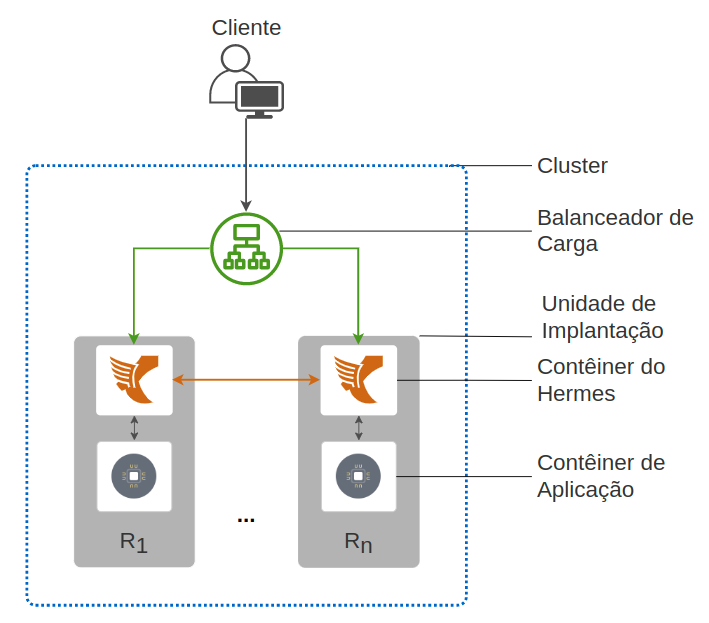
\includegraphics[width=0.8\linewidth]{figures/hermes-overview.png}
{\flushleft Fonte - \textcite{renan2021hermes}}
\label{fig:hermes-architecture}
\end{figure}

A Figura \ref{fig:hermes-architecture} mostra a arquitetura do Hermes em orquestrador de contêineres. O contêiner do Hermes se localiza à frente do contêiner de aplicação. O bloco cinza se trata da unidade de implantação, onde podem haver as unidades $R_{1}, R_{2}, R_{3}, \ldots, R_{n}$. A diferença é que quando o cliente envia uma mensagem qualquer para algum serviço, o balanceador de carga irá repassar essa mensagem para um Hermes, esse Hermes fará o papel de interceptar a mensagem e depois irá executar a ordenação de mensagens, uma vez ordenadas as mensagens o Hermes executa a aplicação dessas mensagens nos contêineres da aplicação. Desta maneira se implementa o padrão de projetos Sidecar, pois o Hermes está ao lado do contêiner de aplicação e a comunicação entre os contêineres de Implantação e de Aplicação é feita através de endereço \gls{IP} e porta.

% \textbf{Interface}

% \textbf{Padrão \textit{Interceptor}}

% \textbf{Onde o interceptador se encontra}

A aplicação está contida dentro dos \textit{Pods}, e cada \textit{Pod} tem um Hermes e uma aplicação alvo sendo replicada. As requisições chegam para o Hermes líder que repassa a mensagem em bytes para o Raft poder ordenar usando consenso entre os participantes.

% O Hermes, por sua vez, deve acionar o algoritmo de consenso para poder ordenar as mensagens recebidas. O banco de dados chave valor \textit{etcd} pode ser usado para armazenar informações essenciais para o funcionamento do algoritmo de consenso.

\section{Detalhes de implementação do Hermes}

O desenvolvimento sobre as classes de projeto do Hermes requer que alguns conceitos sejam observados.

\begin{figure}[!htb]
\centering
\caption{Relação entre os componentes do interceptador Hermes}
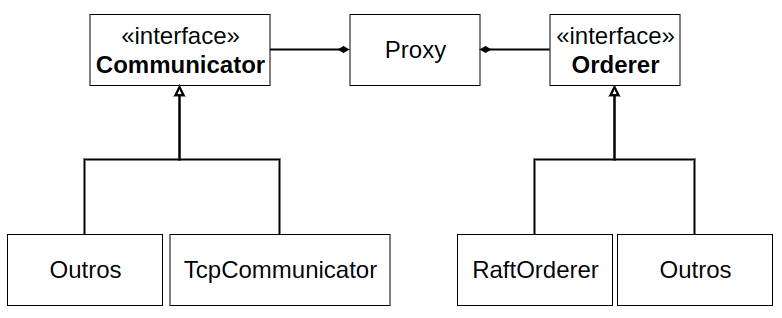
\includegraphics[width=0.9\linewidth]{figures/hermes-components.png}
\label{fig:componentes-hermes}
{\flushleft Fonte - Adaptado de \textcite{renan2021hermes}}
\end{figure}

A Figura \ref{fig:componentes-hermes} mostra a arquitetura do Hermes em UML. O Hermes foi implementado com padrão de projeto Proxy que por sua vez é composto de 2 objetos, sendo um \textit{comunicador} e um \textit{ordenador}. O \textit{comunicador} implementa a interface \textit{Communicator} e o ordenador implementa a interface \textit{Orderer}.

\begin{figure}[!htb]
\centering
\caption{Interfaces do código Hermes}
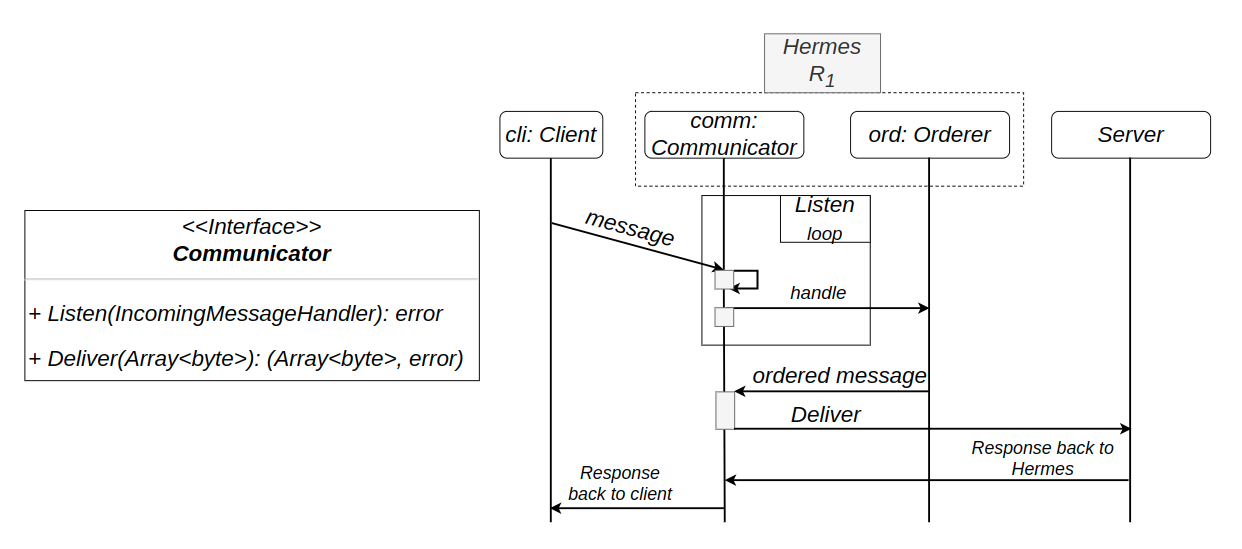
\includegraphics[width=\linewidth]{figures/communicator.drawio.png}
{\flushleft Fonte - Adaptado de \textcite{renan2021hermes}}
\label{fig:communicator-interfaces-hermes}
\end{figure}

A Figura \ref{fig:communicator-interfaces-hermes} mostra a interface \textit{Communicator} com os métodos \textit{Listen} e \textit{Deliver} ao lado de um diagrama de mensagens para ilustrar o funcionamento da interface. É possível observar que o método \textit{Listen} permanece escutando mensagens do \textit{Client}. Assim que uma mensagem é capturada, transforma-se esta mensagem para bytes e se envia para o \textit{Orderer}, através do método \textit{IncomingMessageHandler} que fora previamente configurada. A parte do \textit{Orderer} está omitida no diagrama, porém o \textit{Orderer} irá processar a mensagem, executando um algoritmo específico de ordenação de mensagens \textit{i.e.} Raft ou Paxos. Depois de ordenar a mensagem, o \textit{Orderer} retorna a mensagem em bytes para o método \textit{Deliver}, o \textit{Deliver} irá trabalhar a mensagem e finalmente envia para o servidor de aplicação, porém com a certeza que a mensagem já foi ordenada. Após isto o Hermes ainda pode receber uma resposta do Servidor replicado e assim o Hermes pode repassar a resposta para o \textit{Client}.

\begin{figure}[!htb]
\centering
\caption{Interfaces do código Hermes}
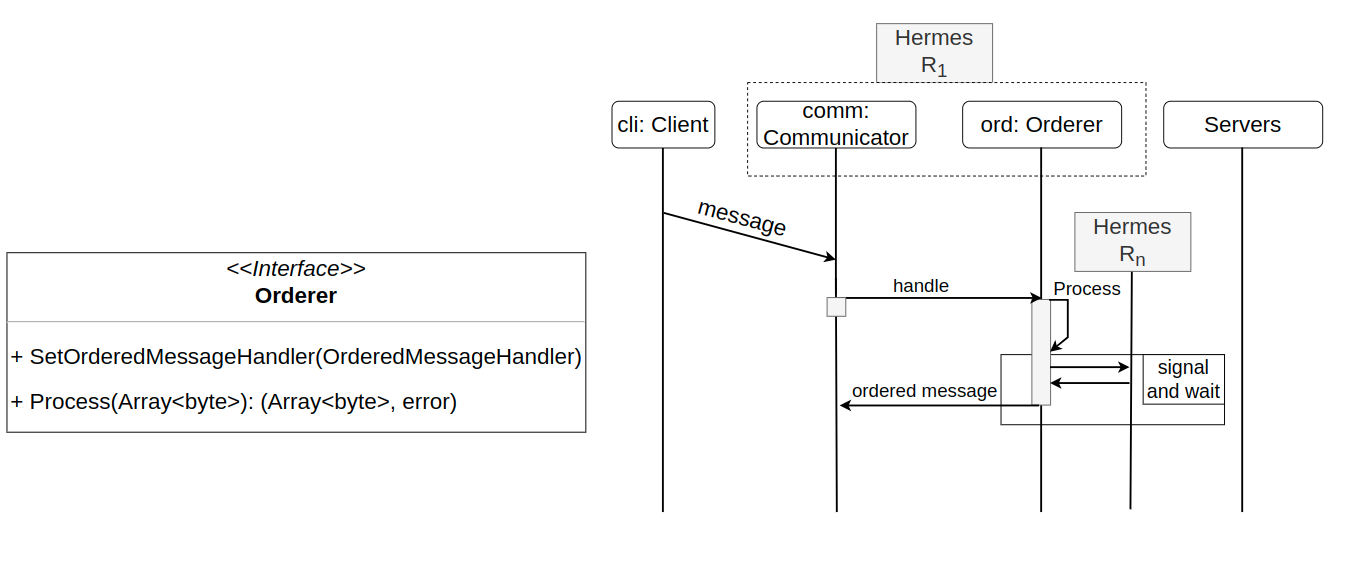
\includegraphics[width=\linewidth]{figures/orderer.drawio.png}
{\flushleft Fonte - Adaptado de \textcite{renan2021hermes}}
\label{fig:orderer-interfaces-hermes}
\end{figure}

A Figura \ref{fig:orderer-interfaces-hermes} mostra a interface \textit{Orderer} com os métodos \textit{SetOrdererMessageHandler} e \textit{Process} ao lado de um diagrama de mensagens para ilustrar o funcionamento da interface. Focando no \textit{Orderer}, assim que a mensagem chega para o \textit{Orderer} através do método IncomingMessageHandler, essa mensagem será executada pelo método Process que recebe uma mensagem em \textit{bytes}, depois de executar o algoritmo de ordenação e interagir com as outras réplicas de Hermes então será feita a aplicação da mensagem nos servidor de aplicação.
